\documentclass[border=3pt]{standalone}
% Shared preamble for the standalone figures.
\usepackage[T1]{fontenc}
\usepackage[scaled=0.9]{helvet}
\renewcommand{\familydefault}{\sfdefault}
\usepackage{tikz}
\usetikzlibrary{arrows.meta,positioning,calc}

\definecolor{ink}{RGB}{28,28,30}
\definecolor{rule}{RGB}{95,97,104}
\definecolor{muted}{RGB}{112,114,121}
\definecolor{accent}{RGB}{172,56,44}
\definecolor{probfill}{RGB}{250,244,235}
\definecolor{detfill}{RGB}{239,243,247}

\newcommand{\zone}[1]{{\fontsize{6.6}{8}\selectfont\bfseries #1}}
\newcommand{\sub}[1]{{\fontsize{7.2}{9}\selectfont\color{muted}#1}}
\newcommand{\mono}[1]{{\fontencoding{OT1}\fontfamily{cmtt}\selectfont #1}}

\tikzset{
  every picture/.style={font=\fontsize{8}{10}\selectfont, text=ink,
    >={Stealth[length=4.6pt,width=3.8pt]}},
  box/.style={draw=rule, line width=0.5pt, rounded corners=2pt, fill=white,
    minimum height=8mm, minimum width=16mm, inner sep=2pt, align=center},
  flow/.style={->, draw=rule, line width=0.6pt},
  hot/.style={->, draw=accent, line width=0.9pt},
  lbl/.style={font=\fontsize{7.2}{9}\selectfont, text=muted, inner sep=1.5pt},
}

\begin{document}
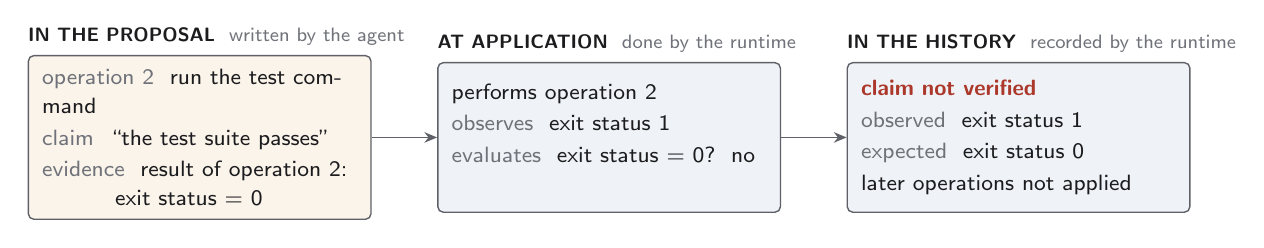
\begin{tikzpicture}
\tikzset{
  panel/.style={draw=rule, line width=0.5pt, rounded corners=2pt, fill=white,
    text width=40mm, minimum height=19mm, inner sep=5pt, align=left,
    font=\fontsize{7.6}{10.4}\selectfont},
  head/.style={font=\fontsize{6.6}{8}\selectfont\bfseries, anchor=south west, inner sep=0pt},
  k/.style={},
}
\node[panel, fill=probfill] (a) at (0,0) {%
  \textcolor{muted}{operation 2}\ \ run the test command\\[1pt]
  \textcolor{muted}{claim}\ \ ``the test suite passes''\\[1pt]
  \textcolor{muted}{evidence}\ \ result of operation 2:\\
  \hspace*{3.1em}exit status = 0};
\node[panel, fill=detfill] (b) at (5.2,0) {%
  performs operation 2\\[1pt]
  \textcolor{muted}{observes}\ \ exit status 1\\[1pt]
  \textcolor{muted}{evaluates}\ \ exit status = 0?\ \ no\\
  \mbox{}};
\node[panel, fill=detfill] (c) at (10.4,0) {%
  \textbf{\textcolor{accent}{claim not verified}}\\[1pt]
  \textcolor{muted}{observed}\ \ exit status 1\\[1pt]
  \textcolor{muted}{expected}\ \ exit status 0\\[1pt]
  later operations not applied};

\node[head] at ($(a.north west)+(0,0.12)$) {IN THE PROPOSAL \textcolor{muted}{\mdseries\ written by the agent}};
\node[head] at ($(b.north west)+(0,0.12)$) {AT APPLICATION \textcolor{muted}{\mdseries\ done by the runtime}};
\node[head] at ($(c.north west)+(0,0.12)$) {IN THE HISTORY \textcolor{muted}{\mdseries\ recorded by the runtime}};

\draw[flow] (a) -- (b);
\draw[flow] (b) -- (c);
\end{tikzpicture}
\end{document}
